\documentclass[12pt,letterpaper]{article}
\usepackage{graphicx,textcomp}
\usepackage{natbib}
\usepackage{setspace}
\usepackage{fullpage}
\usepackage{color}
\usepackage[reqno]{amsmath}
\usepackage{amsthm}
\usepackage{fancyvrb}
\usepackage{amssymb,enumerate}
\usepackage[all]{xy}
\usepackage{endnotes}
\usepackage{lscape}
\newtheorem{com}{Comment}
\usepackage{float}
\usepackage{hyperref}
\newtheorem{lem} {Lemma}
\newtheorem{prop}{Proposition}
\newtheorem{thm}{Theorem}
\newtheorem{defn}{Definition}
\newtheorem{cor}{Corollary}
\newtheorem{obs}{Observation}
\usepackage[compact]{titlesec}
\usepackage{dcolumn}
\usepackage{tikz}
\usetikzlibrary{arrows}
\usepackage{multirow}
\usepackage{xcolor}
\newcolumntype{.}{D{.}{.}{-1}}
\newcolumntype{d}[1]{D{.}{.}{#1}}
\definecolor{light-gray}{gray}{0.65}
\usepackage{url}
\usepackage{listings}
\usepackage{color}

\definecolor{codegreen}{rgb}{0,0.6,0}
\definecolor{codegray}{rgb}{0.5,0.5,0.5}
\definecolor{codepurple}{rgb}{0.58,0,0.82}
\definecolor{backcolour}{rgb}{0.95,0.95,0.92}

\lstdefinestyle{mystyle}{
	backgroundcolor=\color{backcolour},   
	commentstyle=\color{codegreen},
	keywordstyle=\color{magenta},
	numberstyle=\tiny\color{codegray},
	stringstyle=\color{codepurple},
	basicstyle=\footnotesize,
	breakatwhitespace=false,         
	breaklines=true,                 
	captionpos=b,                    
	keepspaces=true,                 
	numbers=left,                    
	numbersep=5pt,                  
	showspaces=false,                
	showstringspaces=false,
	showtabs=false,                  
	tabsize=2
}
\lstset{style=mystyle}
\newcommand{\Sref}[1]{Section~\ref{#1}}
\newtheorem{hyp}{Hypothesis}

\title{Problem Set 1}
\date{Due: September 30, 2024}
\author{Applied Stats/Quant Methods 1}


\begin{document}
	\maketitle
	
	\section*{Instructions}
	\begin{itemize}
		\item Please show your work! You may lose points by simply writing in the answer. If the problem requires you to execute commands in \texttt{R}, please include the code you used to get your answers. Please also include the \texttt{.R} file that contains your code. If you are not sure if work needs to be shown for a particular problem, please ask.
		\item Your homework should be submitted electronically on GitHub.
		\item This problem set is due before 23:59 on Monday September 30, 2024. No late assignments will be accepted.
		%\item Total available points for this homework is 80.
	\end{itemize}
	
	\vspace{1cm}
	\section*{Question 1: Education}
	
	A school counselor was curious about the average of IQ of the students in her school and took a random sample of 25 students' IQ scores. The following is the data set:\\
	\vspace{.1cm} 
	
	\begin{enumerate}
		
		\item Find a 90\% confidence interval for the average student IQ in the school.\\
		
		\noindent 
		Based on the results of this analysis, we can say that we are 90 percent confident that the  average IQ of the student population lies between 94.13 and 102.75.  
		In order to arrive at this answer, I did the following:\\ 
		\vspace{.2cm}  
		1. I calculated the sample mean which is 98.44\\
		\vspace{.2cm} 
		2. I then calculate the sample standard deviation\\ 
		\vspace{.2cm} 
		3. The standard deviation is approximately 13.09. This tells is the varience of our sample. \\
		\vspace{.2cm} 
		4. I found the z-score associated with the 90 percent confidence interval which is 1.645. This value comes from the standard normal distribution, where 90 percent of the distribution lies within 1.645 standard deviations from the mean whereby leaving 5 percent in each tail. 
		
		
		Please see the following code I used to arrive at this confidence interval.
		
	\lstinputlisting[language=R, firstline=1, lastline=43]{Problem Set 1 Solution.R} 
		
		\vspace{1cm}
		\newpage 
		
		\item Next, the school counselor was curious  whether  the average student IQ in her school is higher than the average IQ score (100) among all the schools in the country.\\ 
		
		
		\noindent Using the same sample, conduct the appropriate hypothesis test with $\alpha=0.05$.
	\end{enumerate}
	

	Based on the results, I think we can conclude that the p-value is 0.7215 which is greater than the significance level of 0.05 which means what we cannot reject the null hypothesis. Alternatively put, there is insufficient evidence to suggest that the school counselor is correct in her hypothesis that the mean IQ of students in their school is higher than that of the country. Instead, there is evidence to suggest that the mean IQ of the sample is lower than or equal to 100.\\ 

	\lstinputlisting[language=R, firstline=43, lastline=87]{Problem Set 1 Solution.R} 
	\newpage
	
	\section*{Question 2: Political Economy}
	
	\noindent Researchers are curious about what affects the amount of money communities spend on addressing homelessness. The following variables constitute our data set about social welfare expenditures in the USA. \\
	\vspace{.5cm}
	
	
	\begin{tabular}{r|l}
		\texttt{State} &\emph{50 states in US} \\
		\texttt{Y} & \emph{per capita expenditure on shelters/housing assistance in state}\\
		\texttt{X1} &\emph{per capita personal income in state} \\
		\texttt{X2} &  \emph{Number of residents per 100,000 that are "financially insecure" in state}\\
		\texttt{X3} &  \emph{Number of people per thousand residing in urban areas in state} \\
		\texttt{Region} &  \emph{1=Northeast, 2= North Central, 3= South, 4=West} \\
	\end{tabular}
	
	\vspace{.5cm}
	\noindent Explore the \texttt{expenditure} data set and import data into \texttt{R}.
	\vspace{.5cm}
	\vspace{.5cm}
	\begin{itemize}
		
		\item
		Please plot the relationships among \emph{Y}, \emph{X1}, \emph{X2}, and \emph{X3}? What are the correlations among them (you just need to describe the graph and the relationships among them)?
		
		\centering
	
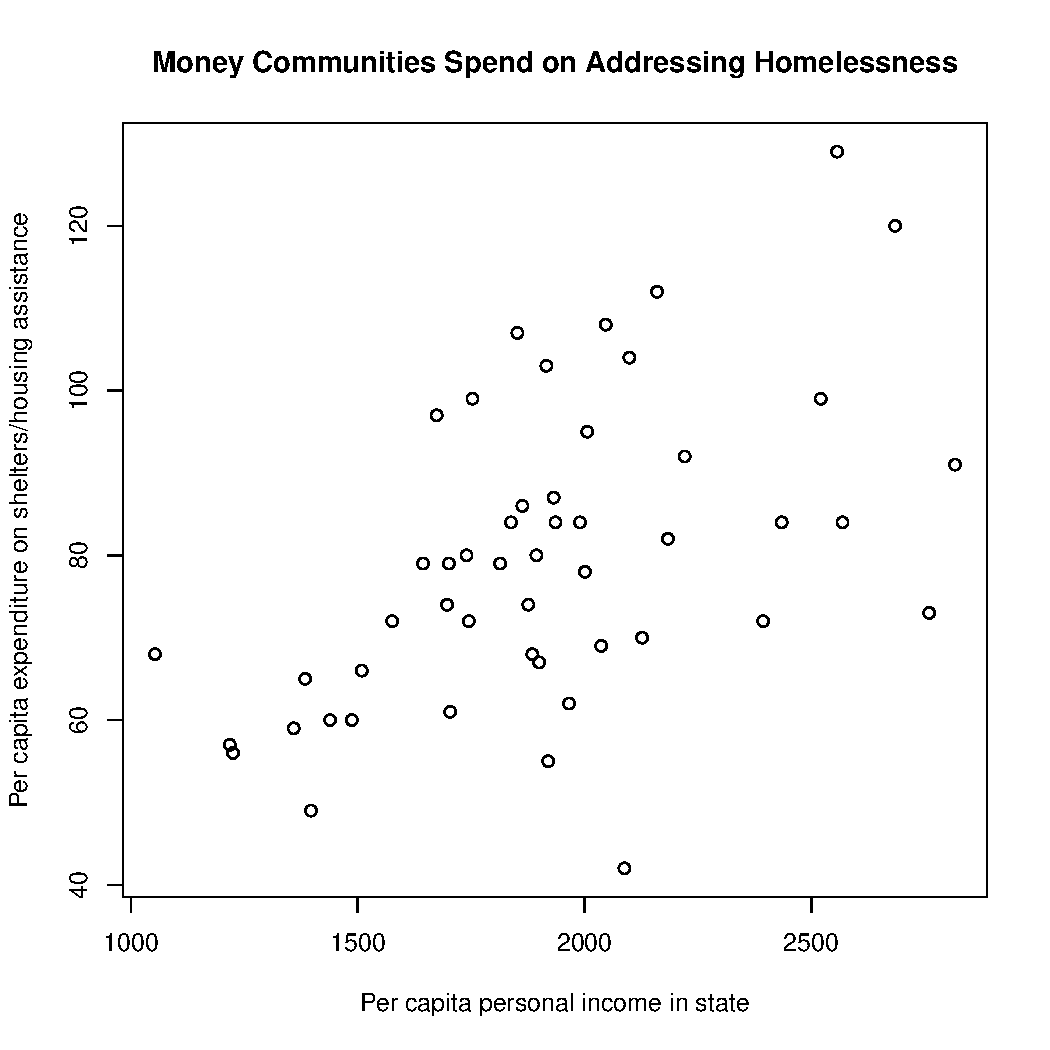
\includegraphics[width=0.8\textwidth]{Y_X1PDF.pdf}
	\vspace{.5cm}
	
		\raggedright
This scatterplot shows us that there is a generally positive association between the per capita personal income and its associated spending on housing assistance (i.e., as personal income per capita increases, so too does the per capita expenditure on housing assistance). However, the observations are spread out, suggesting variability in how different states allocate resources for homelessness despite having similar income levels. This suggests that factors other than income alone influence expenditure levels.
		
	\centering
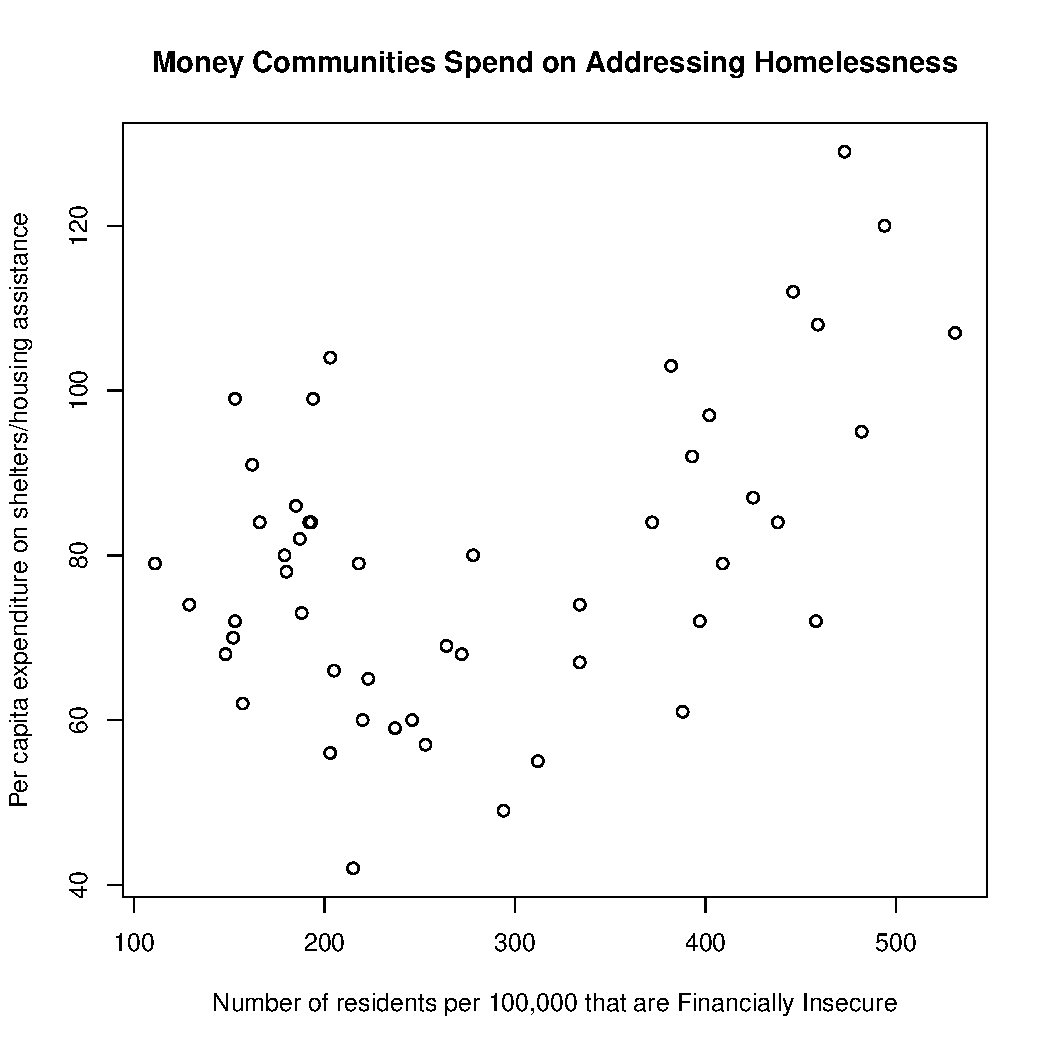
\includegraphics[width=0.8\textwidth]{Y_X2PDF.pdf}
	
		\vspace{.5cm}
		\raggedright
		This scatterplot shows a somewhat unusual distribution and one that doesn't have a strong, directional association. Alternatively put, there doesn't appear to be an assocation between the number of a states inhabilitants that are financially insecure and its associated expenditure on housing assistance. Instead, there is a small cluster of states that have comparatively low numbers of financially insecure residents yet a comparatively high per capita expenditure on housing assistance. 
		
		
	\centering
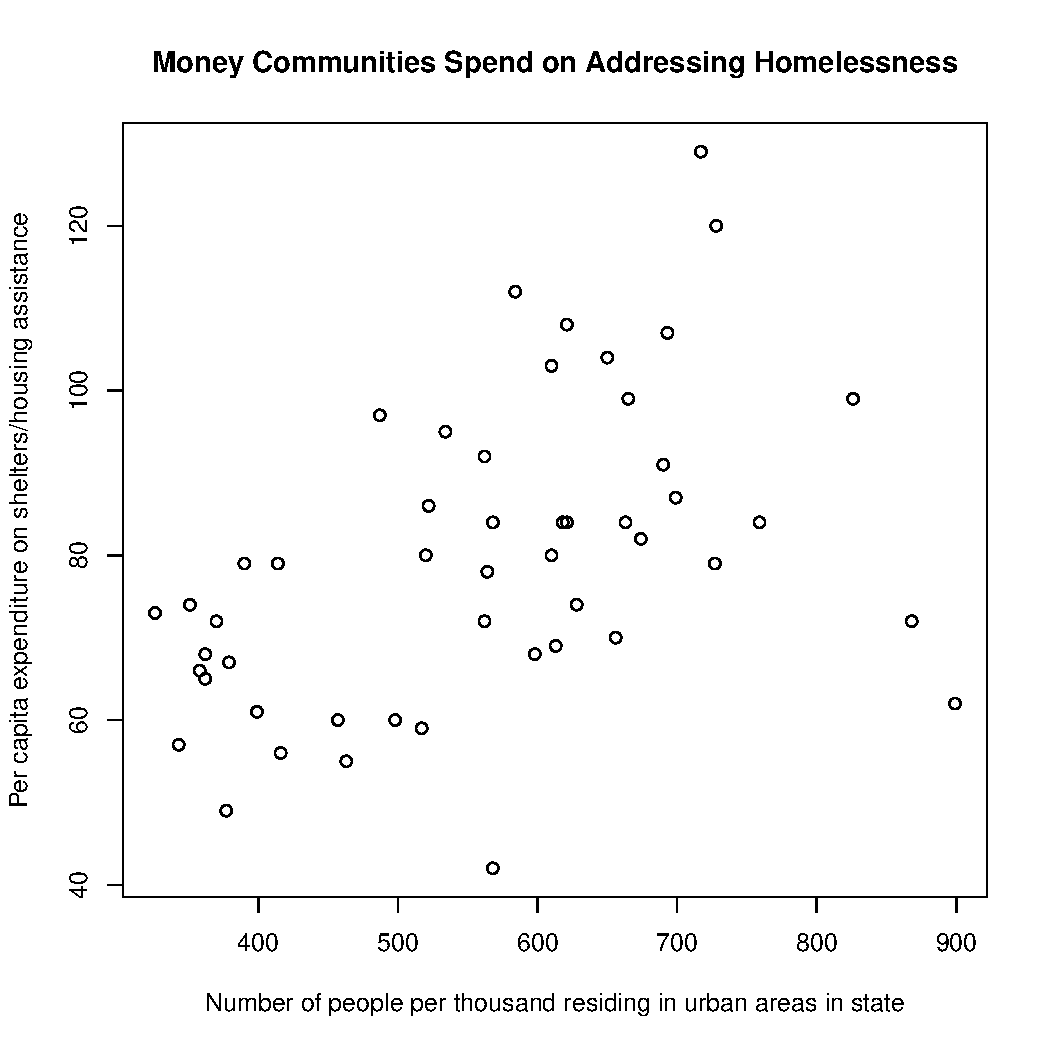
\includegraphics[width=0.8\textwidth]{Y_X3PDF.pdf}

		
		\raggedright
		This scatterplot shows the number of people residing in urban areas in the state and the per capita expenditure on shelter/housing assistance. There appears to be a somewhat positive association between these two variables (i.e. states that have a greater number of urban residents generally have a slightly higher per capita expenditure on shelters and housing assistance) however there is a large amount of variability. There are also a small number of notable outliers, for example, there is one state with an urban resident population of approx 900 thousand with a per capita expenditure of only 64. 

\newpage
		
		\item
		Please plot the relationship between \emph{Y} and \emph{Region}? On average, which region has the highest per capita expenditure on housing assistance?
		\vspace{.5cm}
		
		\centering
	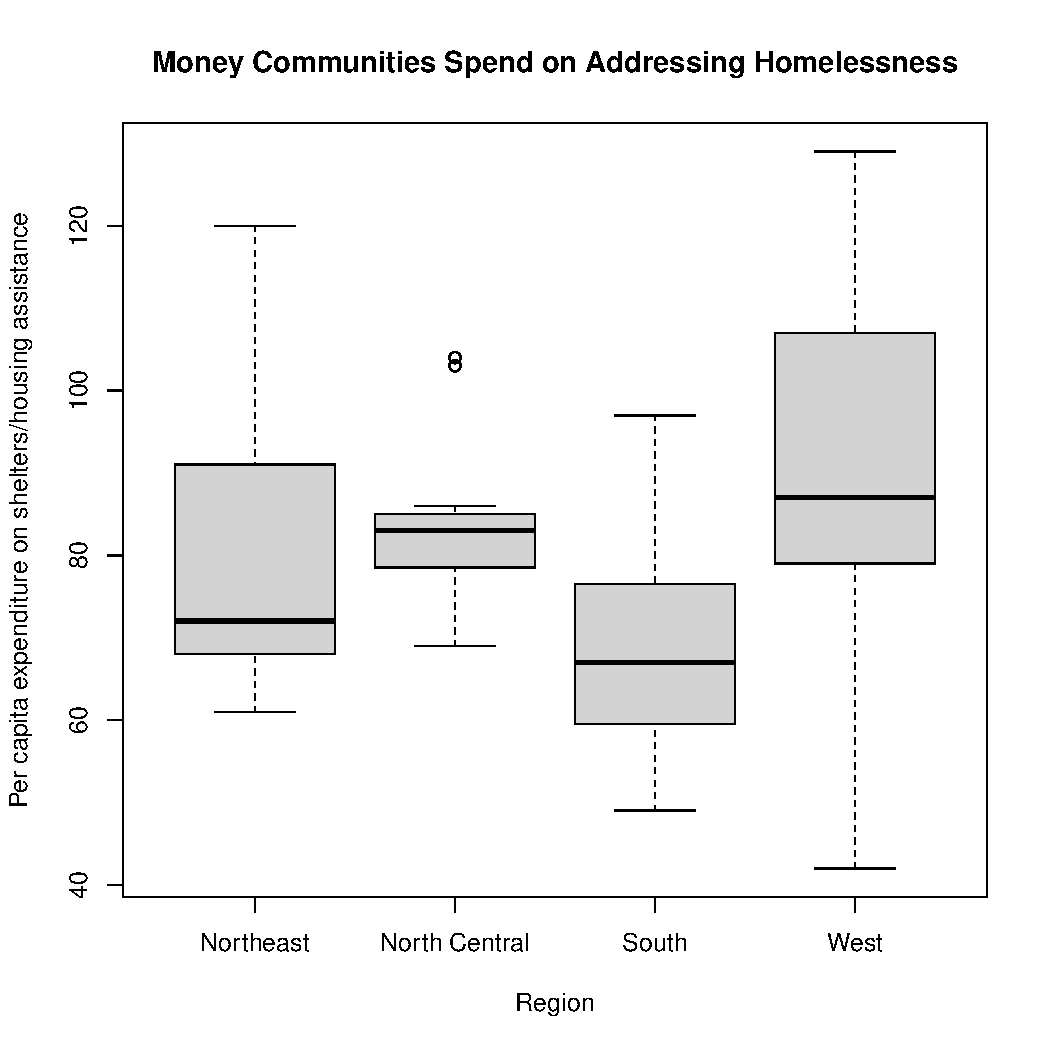
\includegraphics[width=0.8\textwidth]{Y_RegionPDF.pdf}
	
		
		\raggedright
		From the boxplot and assessing the median lines, it appears that the "West" has the highest per captia expenditure on housing assistance. However, the West also has the greatest spread. The "North Central" region has a similar average per capita expenditure but with a significally smaller spread. 
		
		\vspace{.5cm}
		
		The following three graphs map the relationships between the three predictor variables. 
		
\centering
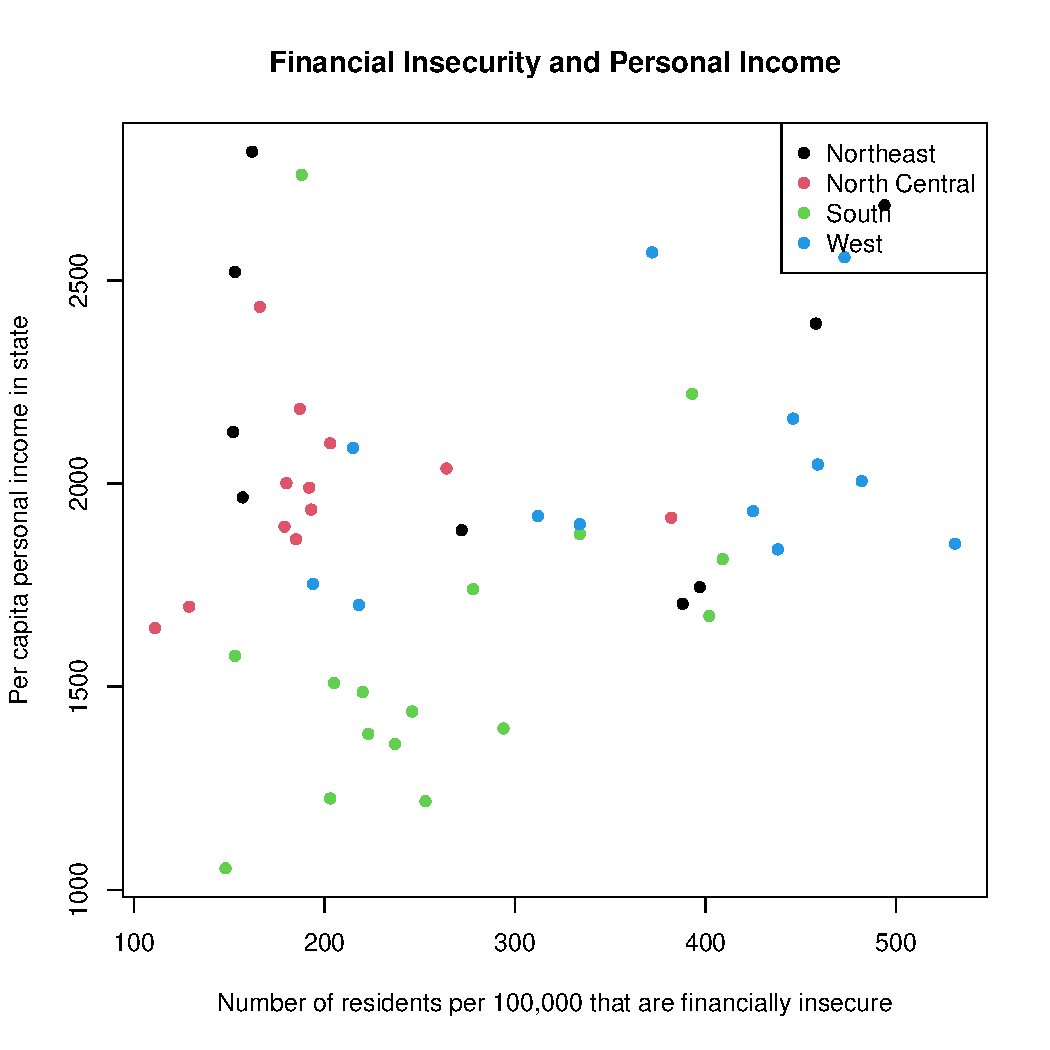
\includegraphics[width=0.8\textwidth]{X1_X2PDF.pdf}

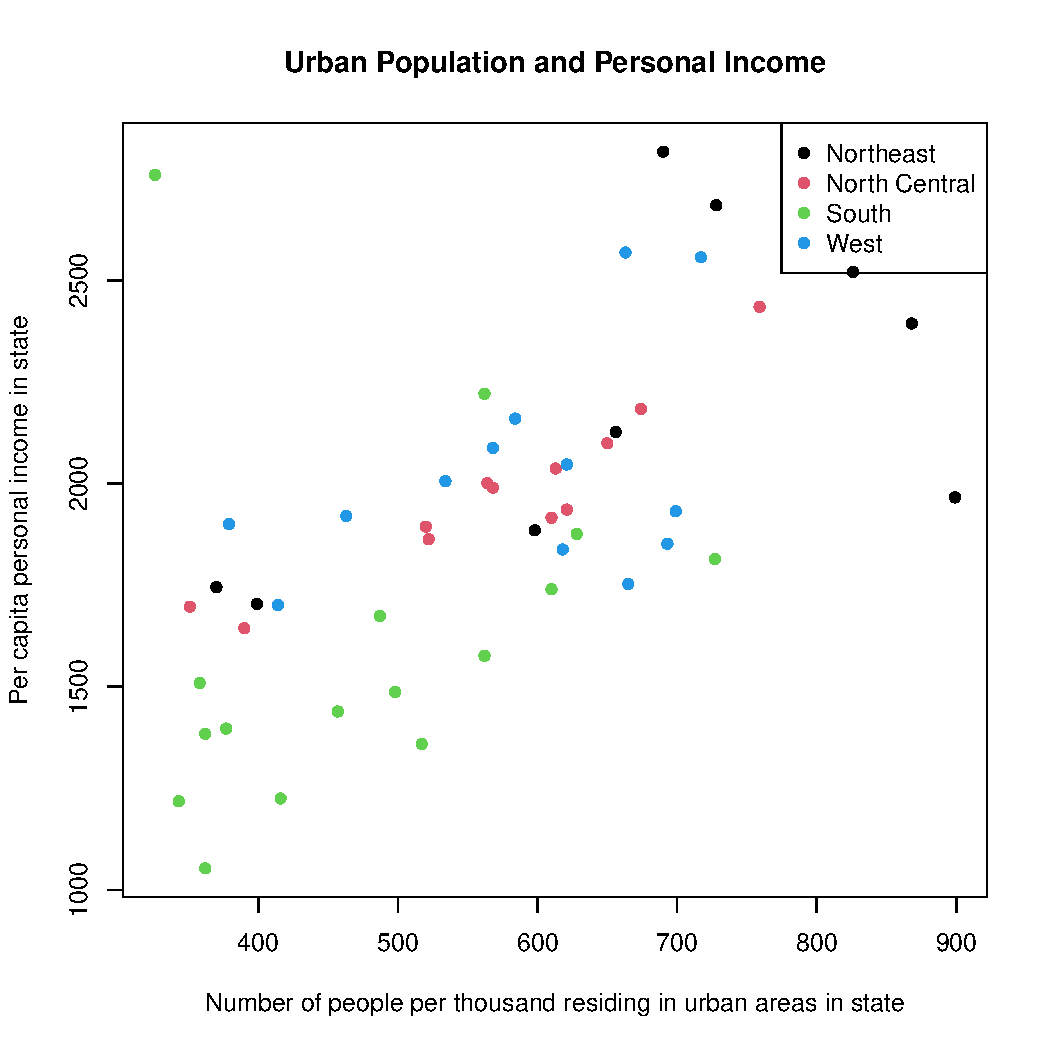
\includegraphics[width=0.8\textwidth]{X1_X3PDF.pdf}

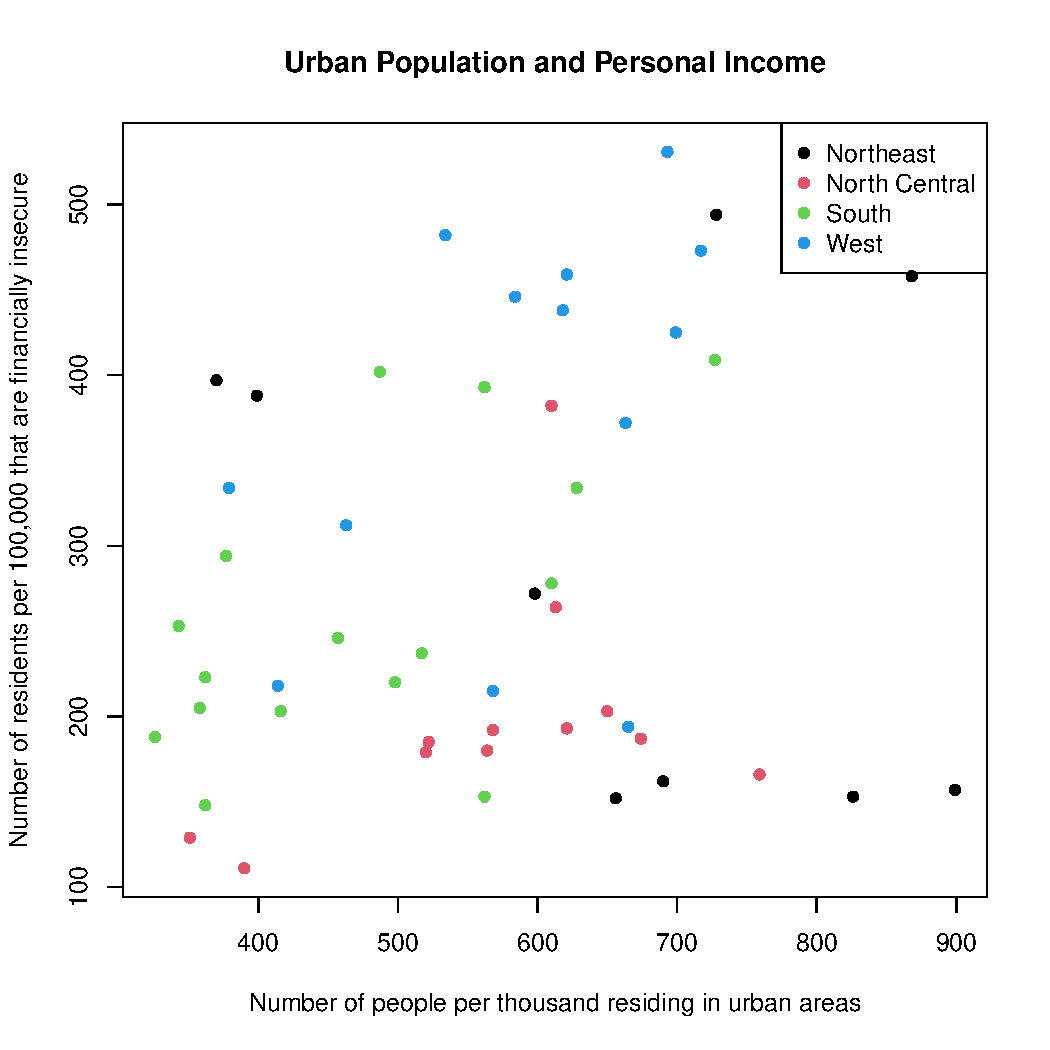
\includegraphics[width=0.8\textwidth]{X2_X3PDF.pdf}
		\newpage
		
		\raggedright
		\item
		Please plot the relationship between \emph{Y} and \emph{X1}? Describe this graph and the relationship. Reproduce the above graph including one more variable \emph{Region} and display different regions with different types of symbols and colors.
		
	\centering
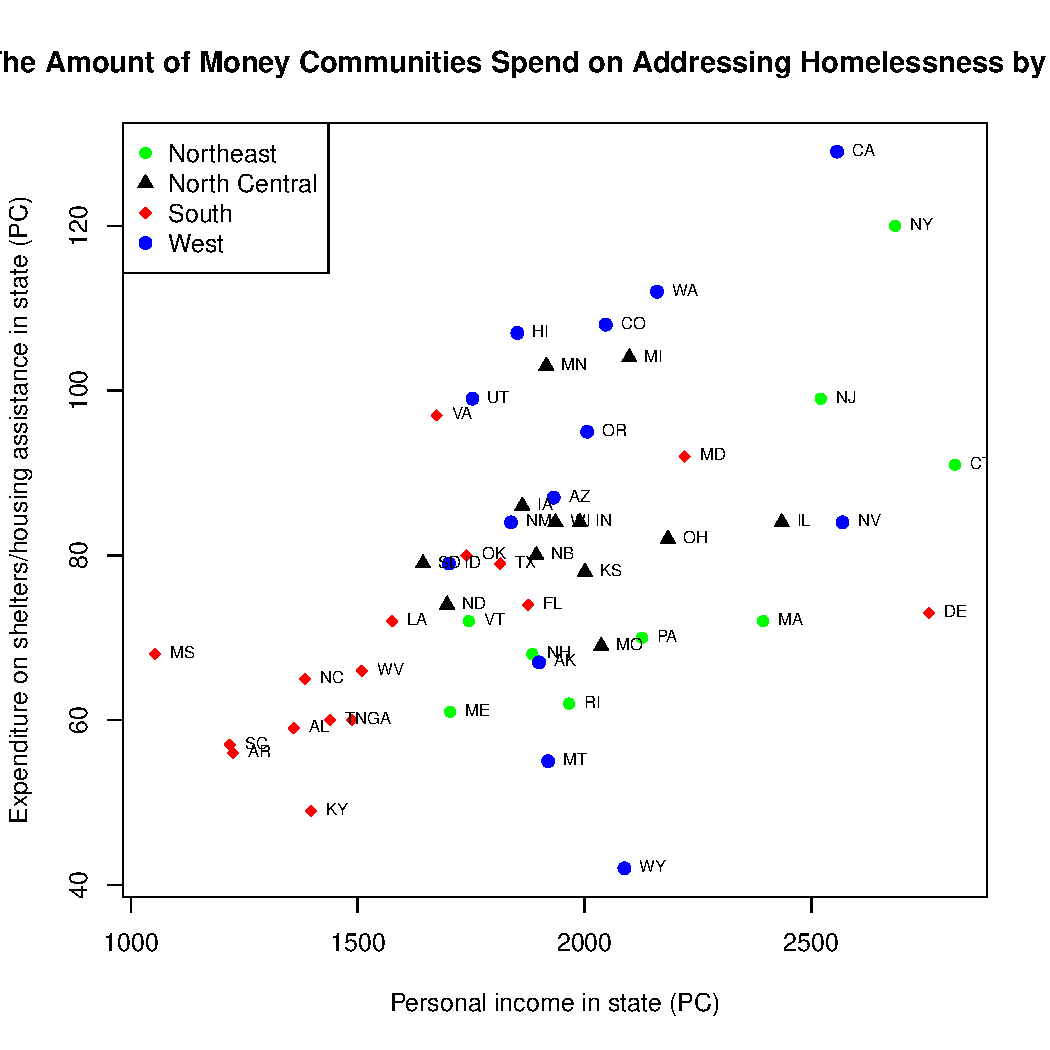
\includegraphics[width=0.8\textwidth]{Final_PlotPDF.pdf}
		
		\raggedright
		From this graph, we can broadly draw the following observations: It appears that the Southern regions of the USA generally have the lowest personal income per capita of the US states (there are exceptions, for example "DE" (Delaware) which is, for some reason, grouped as a Southern state. The states generally appear to have the highest expenditure per capita on housing assistance are those in the "West", "WY" (Wyoming) being a noteworthy outlier. Broadly speaking, we can observe the following from this data visualisation: there is a generally a positive association between per capita personal income and the associated expenditure on housing assistance programs.  
		
		\centering

			\lstinputlisting[language=R, firstline=89, lastline=211]{Problem Set 1 Solution.R} 
		
		
	\end{itemize}
	
	
\end{document}
